\documentclass{article} % For LaTeX2e
\usepackage{url}
\usepackage[
style=authoryear,
backend=bibtex,
]{biblatex}
\usepackage{graphicx}
\graphicspath{ {./Graphics/} }
\usepackage{enumitem}
\usepackage{placeins}
\usepackage{float}

\addbibresource{ProposalBib.bib}

\title{STOR 496 Independent Project Proposal}
\author{
Adam Dameron
}

\begin{document}


\maketitle

\begin{abstract}
This proposal is for a project which seeks to use machine learning and object oriented statistics to model international human trafficking behavior. The goal of this project is to show which aspects of trafficking are most correlated with changes in a nations development. This is for the purposes of informing law enforcement and policy makers of what characteristics to be searching for.
\end{abstract}

\section{Introduction}
	Human trafficking occurs on a global scale, and has been recorded as an international concern since the year 1913 \parencite{Aromaa2007}. Many attempts have been made at defining it, yet these definitions remain unclear and vary greatly. Human trafficking is strongly believed to occur in every country, and victimizes individuals of all ages, genders, and backgrounds \parencite{JacK2012}.\medskip
	
	A major gap in the global understanding of international human trafficking, is in how human trafficking is affected by changes in a country's economic and social development. The United Nations mentions this fact in its "Introduction to Human Trafficking," and describes trafficking as a "multidimensional problem," where a development is applicable \parencite{kangaspunta_2008}. However, there exists very little quantitative analysis into how trafficking and development are connected. This research seeks to provide more insight into what connections exist, if any.
	
	%Possibly Redundant%
	%Despite mounting global concern, there still exists very little data on the matter of human trafficking, and of the data that does exist, much of it is poorly maintained or incomplete \parencite{Aromaa2007}. Fortunately, there are statistical methods of handling missing data, particularly in the fields of epidemiology, and public health \parencite{abraham_russell_2004}; however, these methods have yet to be applied to data that exists on human trafficking, with the intention of modeling long-term shifts in certain aspects of human trafficking.%
	
\section{Background Information}

The trafficking of humans is a multifaceted problem which exists at all levels from local to international \parencite{Aromaa2007, JacK2012}. The United Nations defines human trafficking as “recruitment, transportation, transfer, harboring or receipt of people through force, fraud or deception, with the aim of exploiting them for profit” \parencite{Raymond2002}. In order to truly understand the scope of this problem, one must begin by gaining an understanding of the different types of trafficking, and the reasons why it is such a widespread issue in all locations; irregardless of economic, social, and cultural stability.

\subsection*{Defining Types of Trafficking}

The United States State Department has has a designated "Office To Monitor and Combat Trafficking in Persons" since October of 2001. This office publishes a yearly "Trafficking in Persons Report," and in this report, two types of human trafficking are reported on: sex trafficking, and labor trafficking \parencite{StateDept}.

The U.S. State department defines sex trafficking as
"...activities involved when a trafficker uses force, fraud, or coercion to compel another person to engage in a commercial sex act..." Similarly, labor trafficking is defined as "...activities involved when a trafficker uses force, fraud, or coercion to exploit the labor or services of another person \parencite{StateDept}." Needless to say, these definitions lack depth, and seem vague in nature.

Polaris, a non-profit organization that reports, analyzes, and educates others on the intricacies of human trafficking in the United States. Alternatively to the U.S. State Deparment's two proposed types of human trafficking, Polaris has defined twenty-five different types of human trafficking that are very-much present in the United States. To preface the 80 page report on "The Typology of Modern Slavery," Polaris states: "...the ways humans are exploited differ greatly. Each type has unique strategies for recruiting and controlling victims, and concealing the crime. \parencite{polarisTypology}"

The types of trafficking described by Polaris were based off of over 42,000 reports made to the "Human Trafficking Hotline." The types mentioned range from agricultural work and farming to personal sexual servitude and escort services. However, Polaris notes that most cases of human trafficking will involve more than one type, and even these types may not fit neatly into "sex trafficking" or "labor trafficking" \parencite{polarisTypology}.

In conclusion, there is no neatly defined categories for human trafficking, except the general consensus in academia, law enforcement, and non-profits, seems to be that aside from a few edge cases, most instances of human trafficking unfortunately have to be reduced to being in one of two major categories, as any deviation from this results in inconsistent and contradictory definitions. It is for these reasons that we will attempt to use a different method of classifying human trafficking cases, but is important to recognize the work already done on this topic by powerful entities such as the U.S. Department of State, and a large organization such as Polaris.

\subsection*{United States's Involvement in International Trafficking}

The United States has long been growing into the global economic leader it is today \parencite{USEconPower}. With this increase in global influence comes an increase of international crime within the country's borders. Sex and labor trafficking have both been long-standing issue within the United States. Despite both types of trafficking being present, most media and law enforcement attention has specifically targeted towards sex trafficking, particularly of children \parencite{MediaRep}. Logically we can assume that with the influence the US has on global trade and international crime, that there is are instances of individuals of other citizenships being exploited within the country, and in ways that are not just sex trafficking.

\FloatBarrier

\begin{figure}[H]
	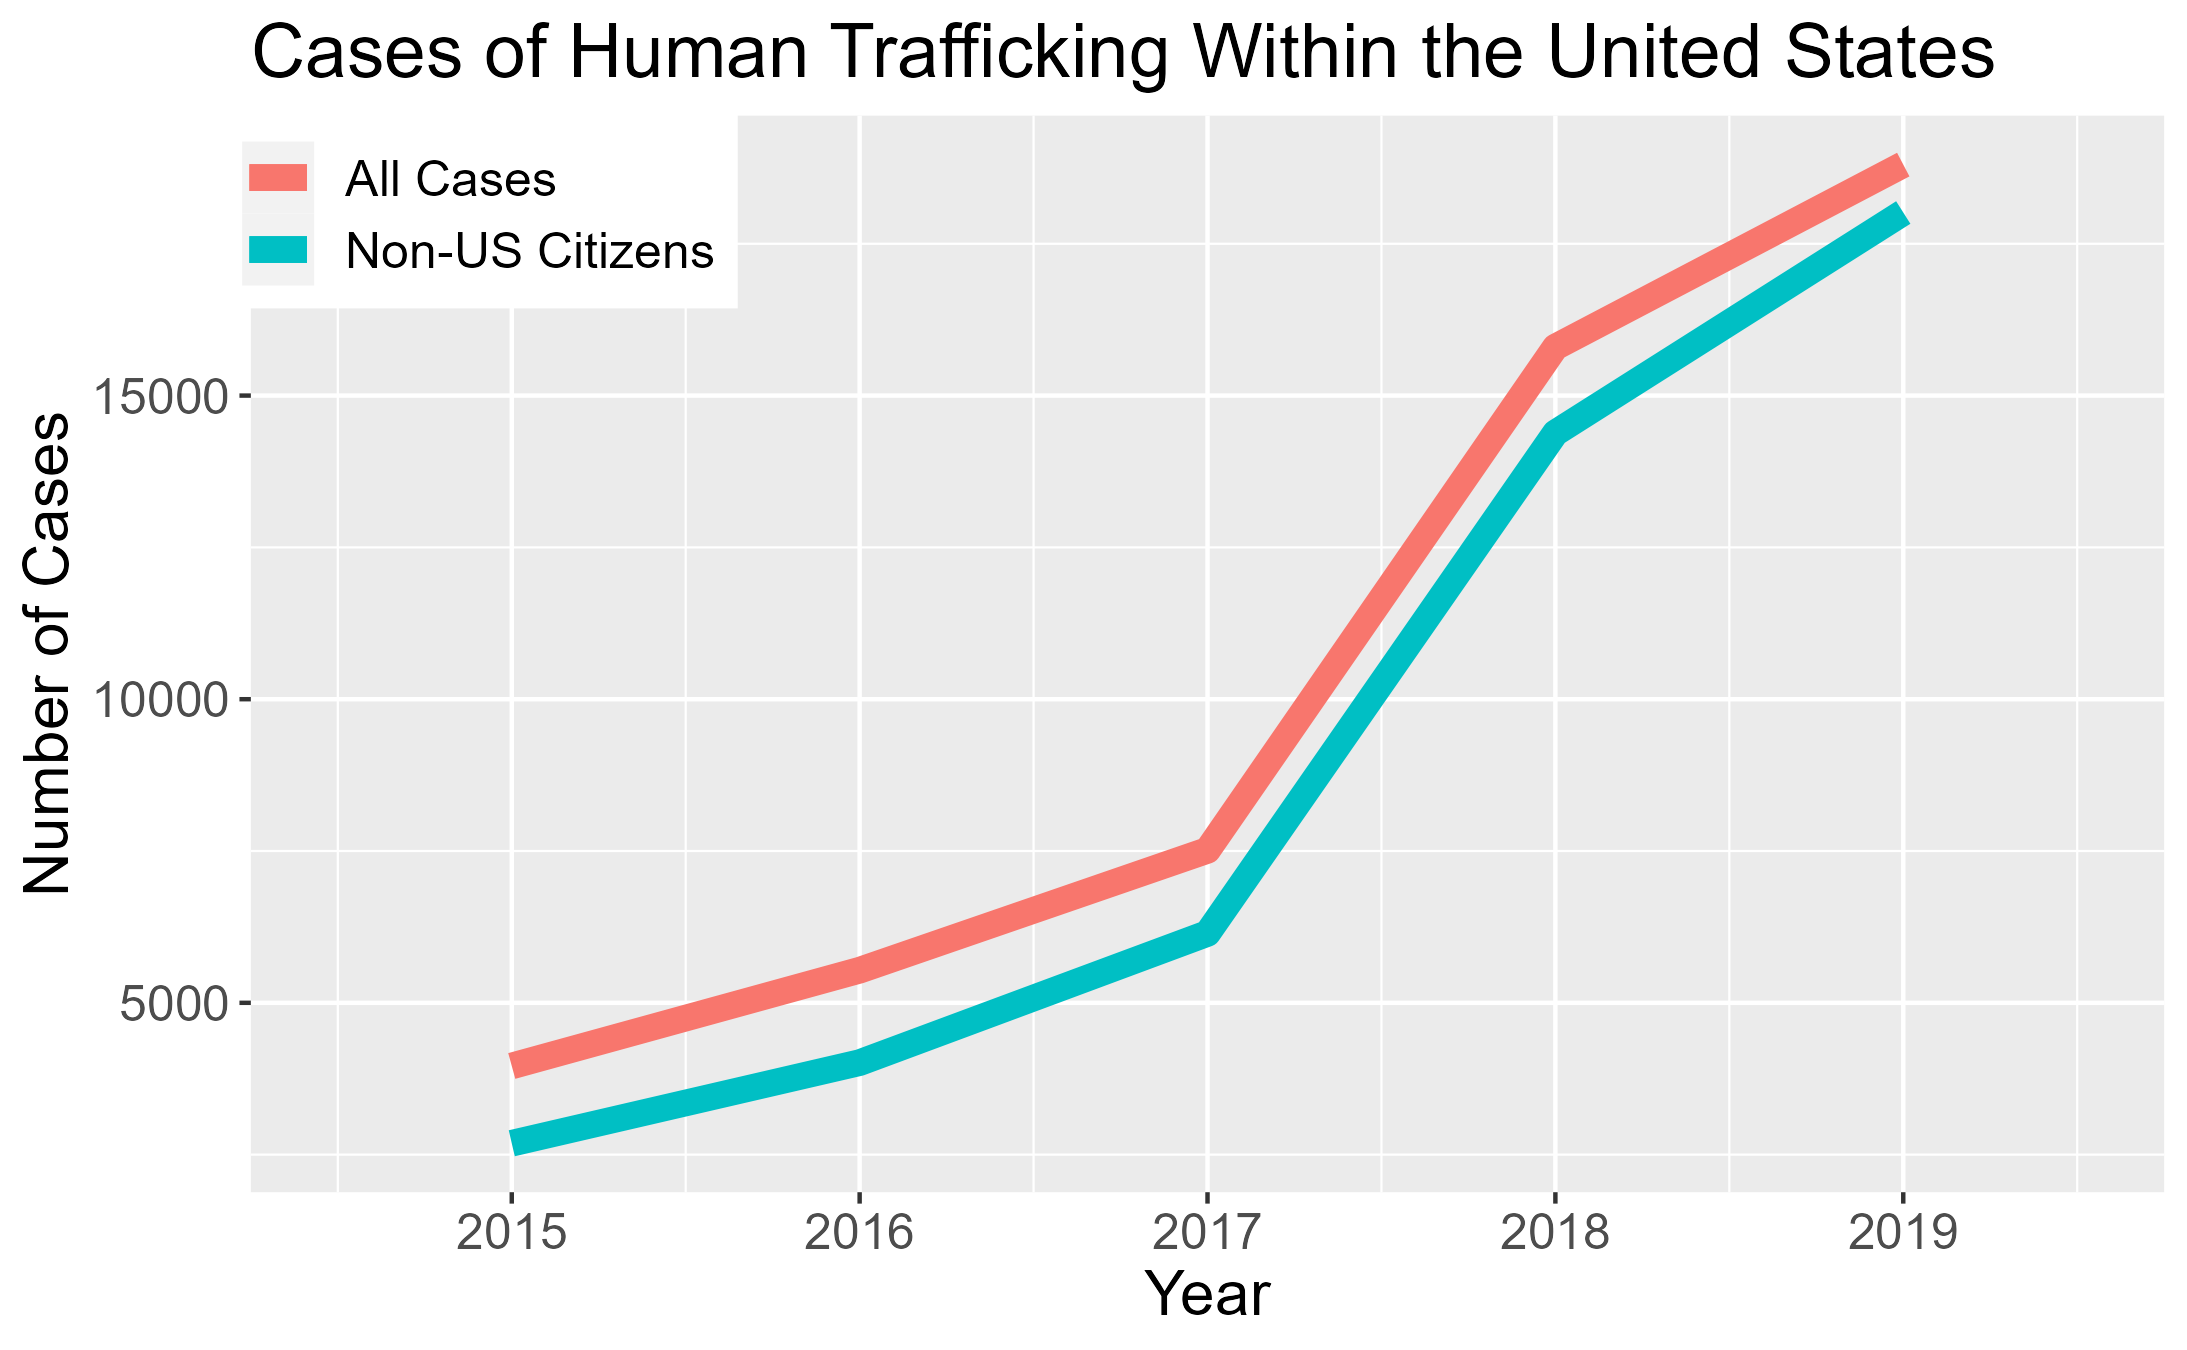
\includegraphics[width = \textwidth]{USTrafficking}
	\scriptsize{\caption{Created with data from \cite{CTDC}}}
\end{figure}

\FloatBarrier

As evidenced in this simple chart, in a span of only 4 years, the number of cases in the United States alone has nearly quadrupled. Although, it is important to note that this is likely to be a severe under-counting of the true number of human trafficking victims each year. Even so, having roughly 20,000 cases in 2019 alone is rather extreme, and shows that this is very much an issue that exists in the United States. Of additional importance is the fact that a large proportion of all cases in the US are ones involving non-US citizens. This means that not only is trafficking present in the US, but international trafficking is of major concern.

\FloatBarrier

\begin{figure}[H]
	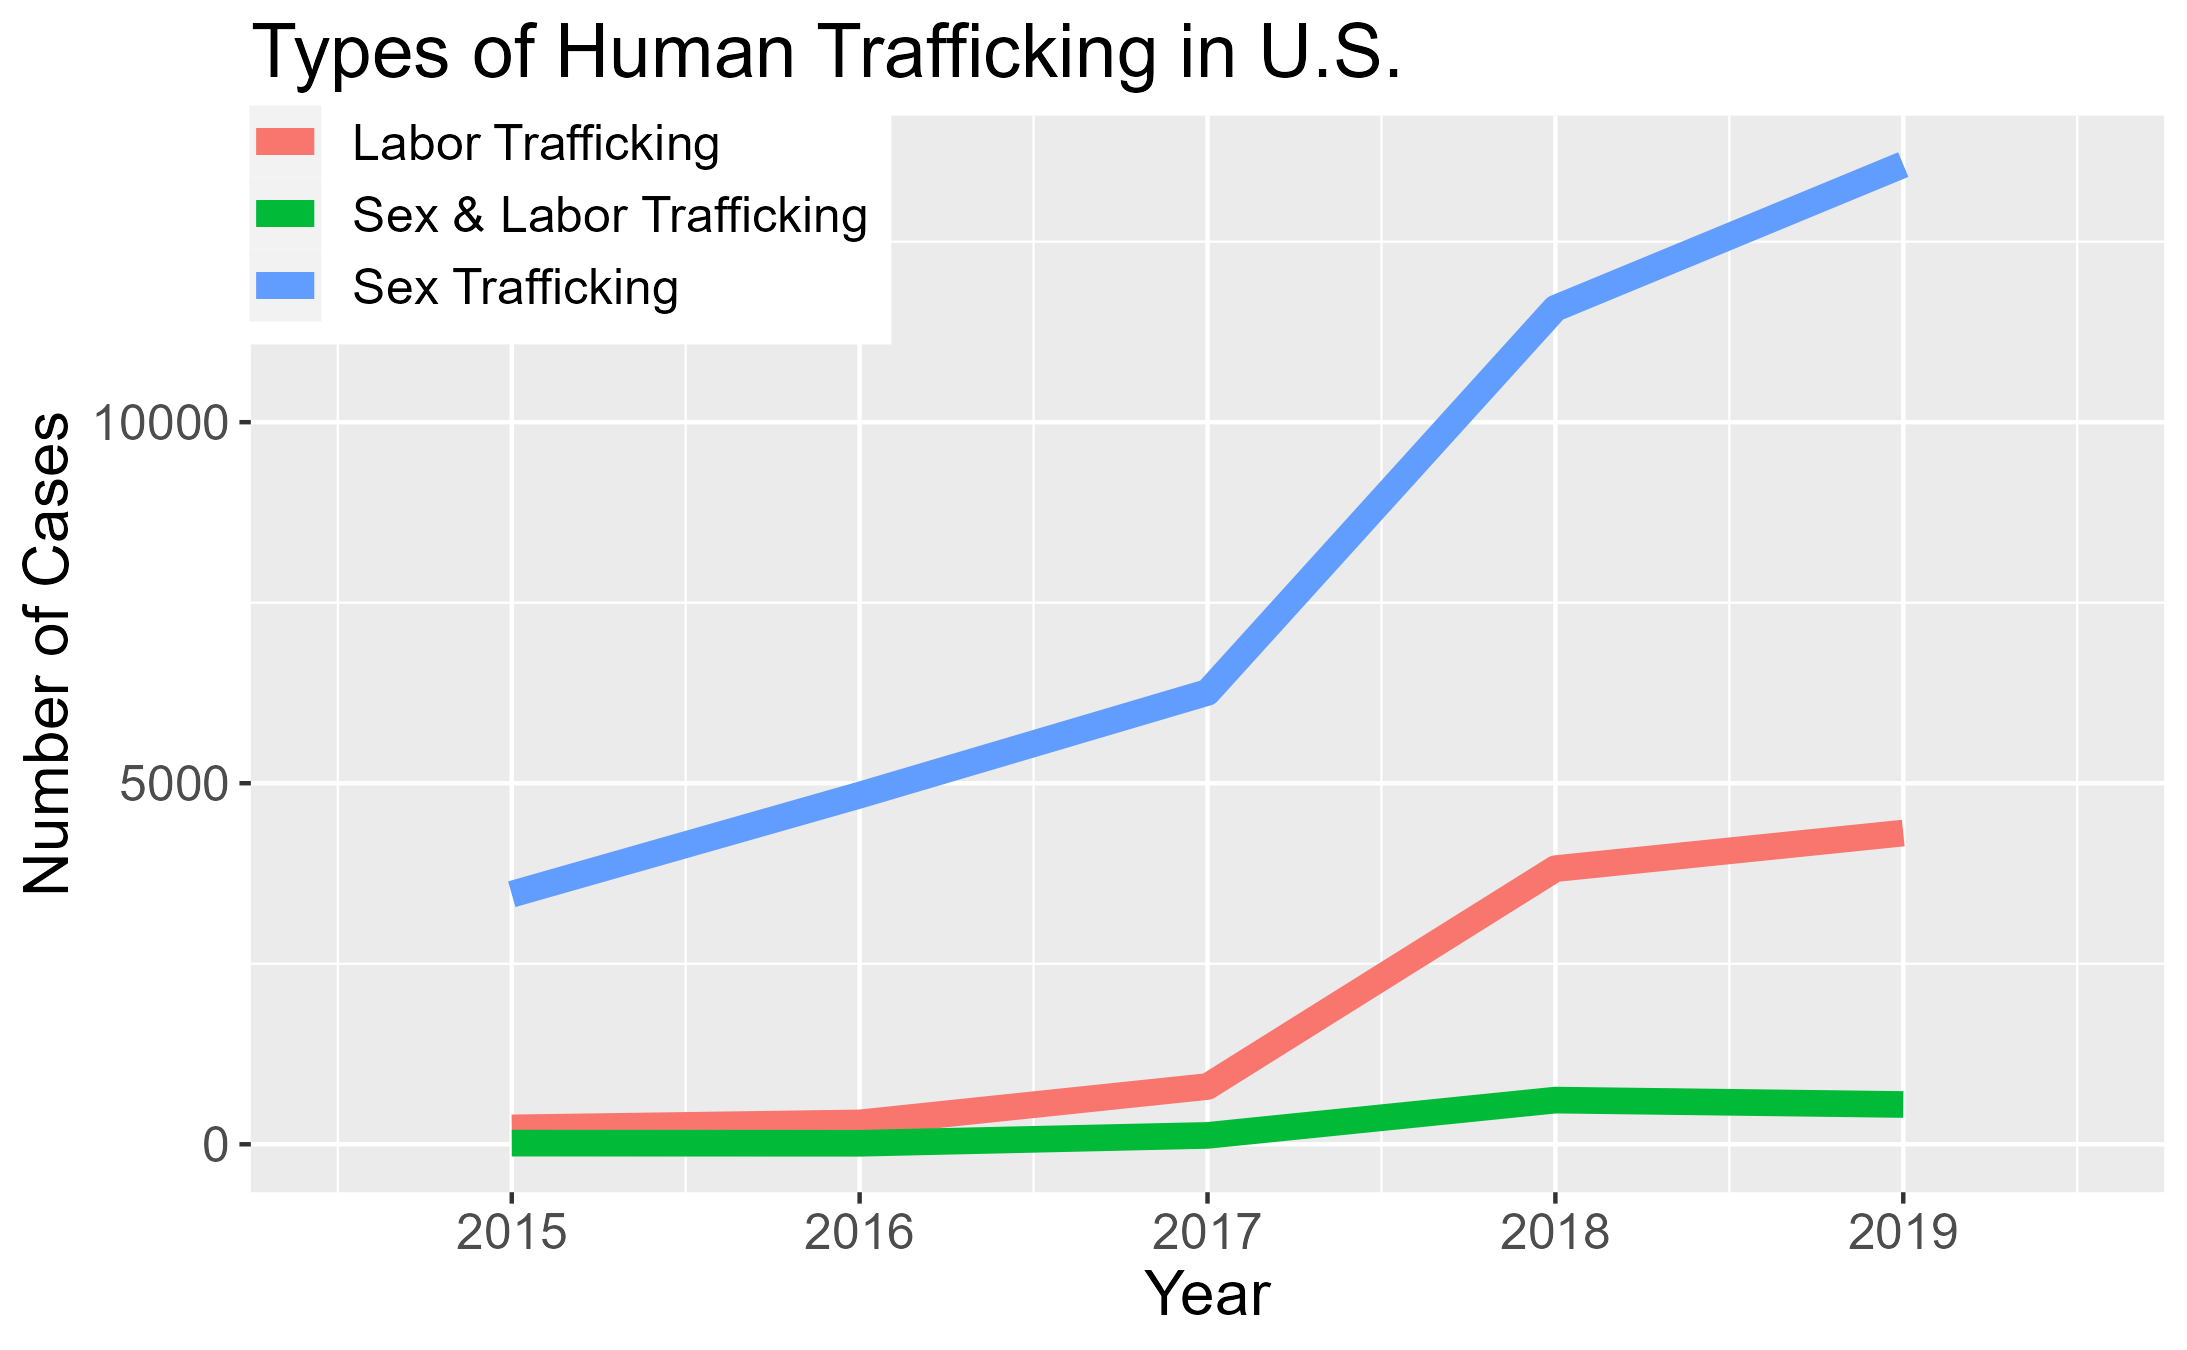
\includegraphics[width = \textwidth]{USTrafficking2}
	\scriptsize{\caption{Created with data from \cite{CTDC}}}
\end{figure}

\FloatBarrier

From this plot, one can see that again, each year there is an increase in the total number of reported cases; however, we see that a significant number of cases exist in which sex trafficking is not the sole type of trafficking present. Thus, even within th U.S., international trafficking is a very real issue, and it exists in all forms, not just sexual. Thus it would be beneficial to better understand, or even predict, what aspects of these victims law enforcement should be knowledgeable of. 

\subsection*{Scale of International Trafficking}

It is difficult to put into words the scale of international human trafficking. However, by looking at the number of human trafficking victims reported in each country, and then determining what percent of them are from other countries, we can visualize the scale of the problem.

\FloatBarrier

\begin{center}
	\begin{figure}[H]
		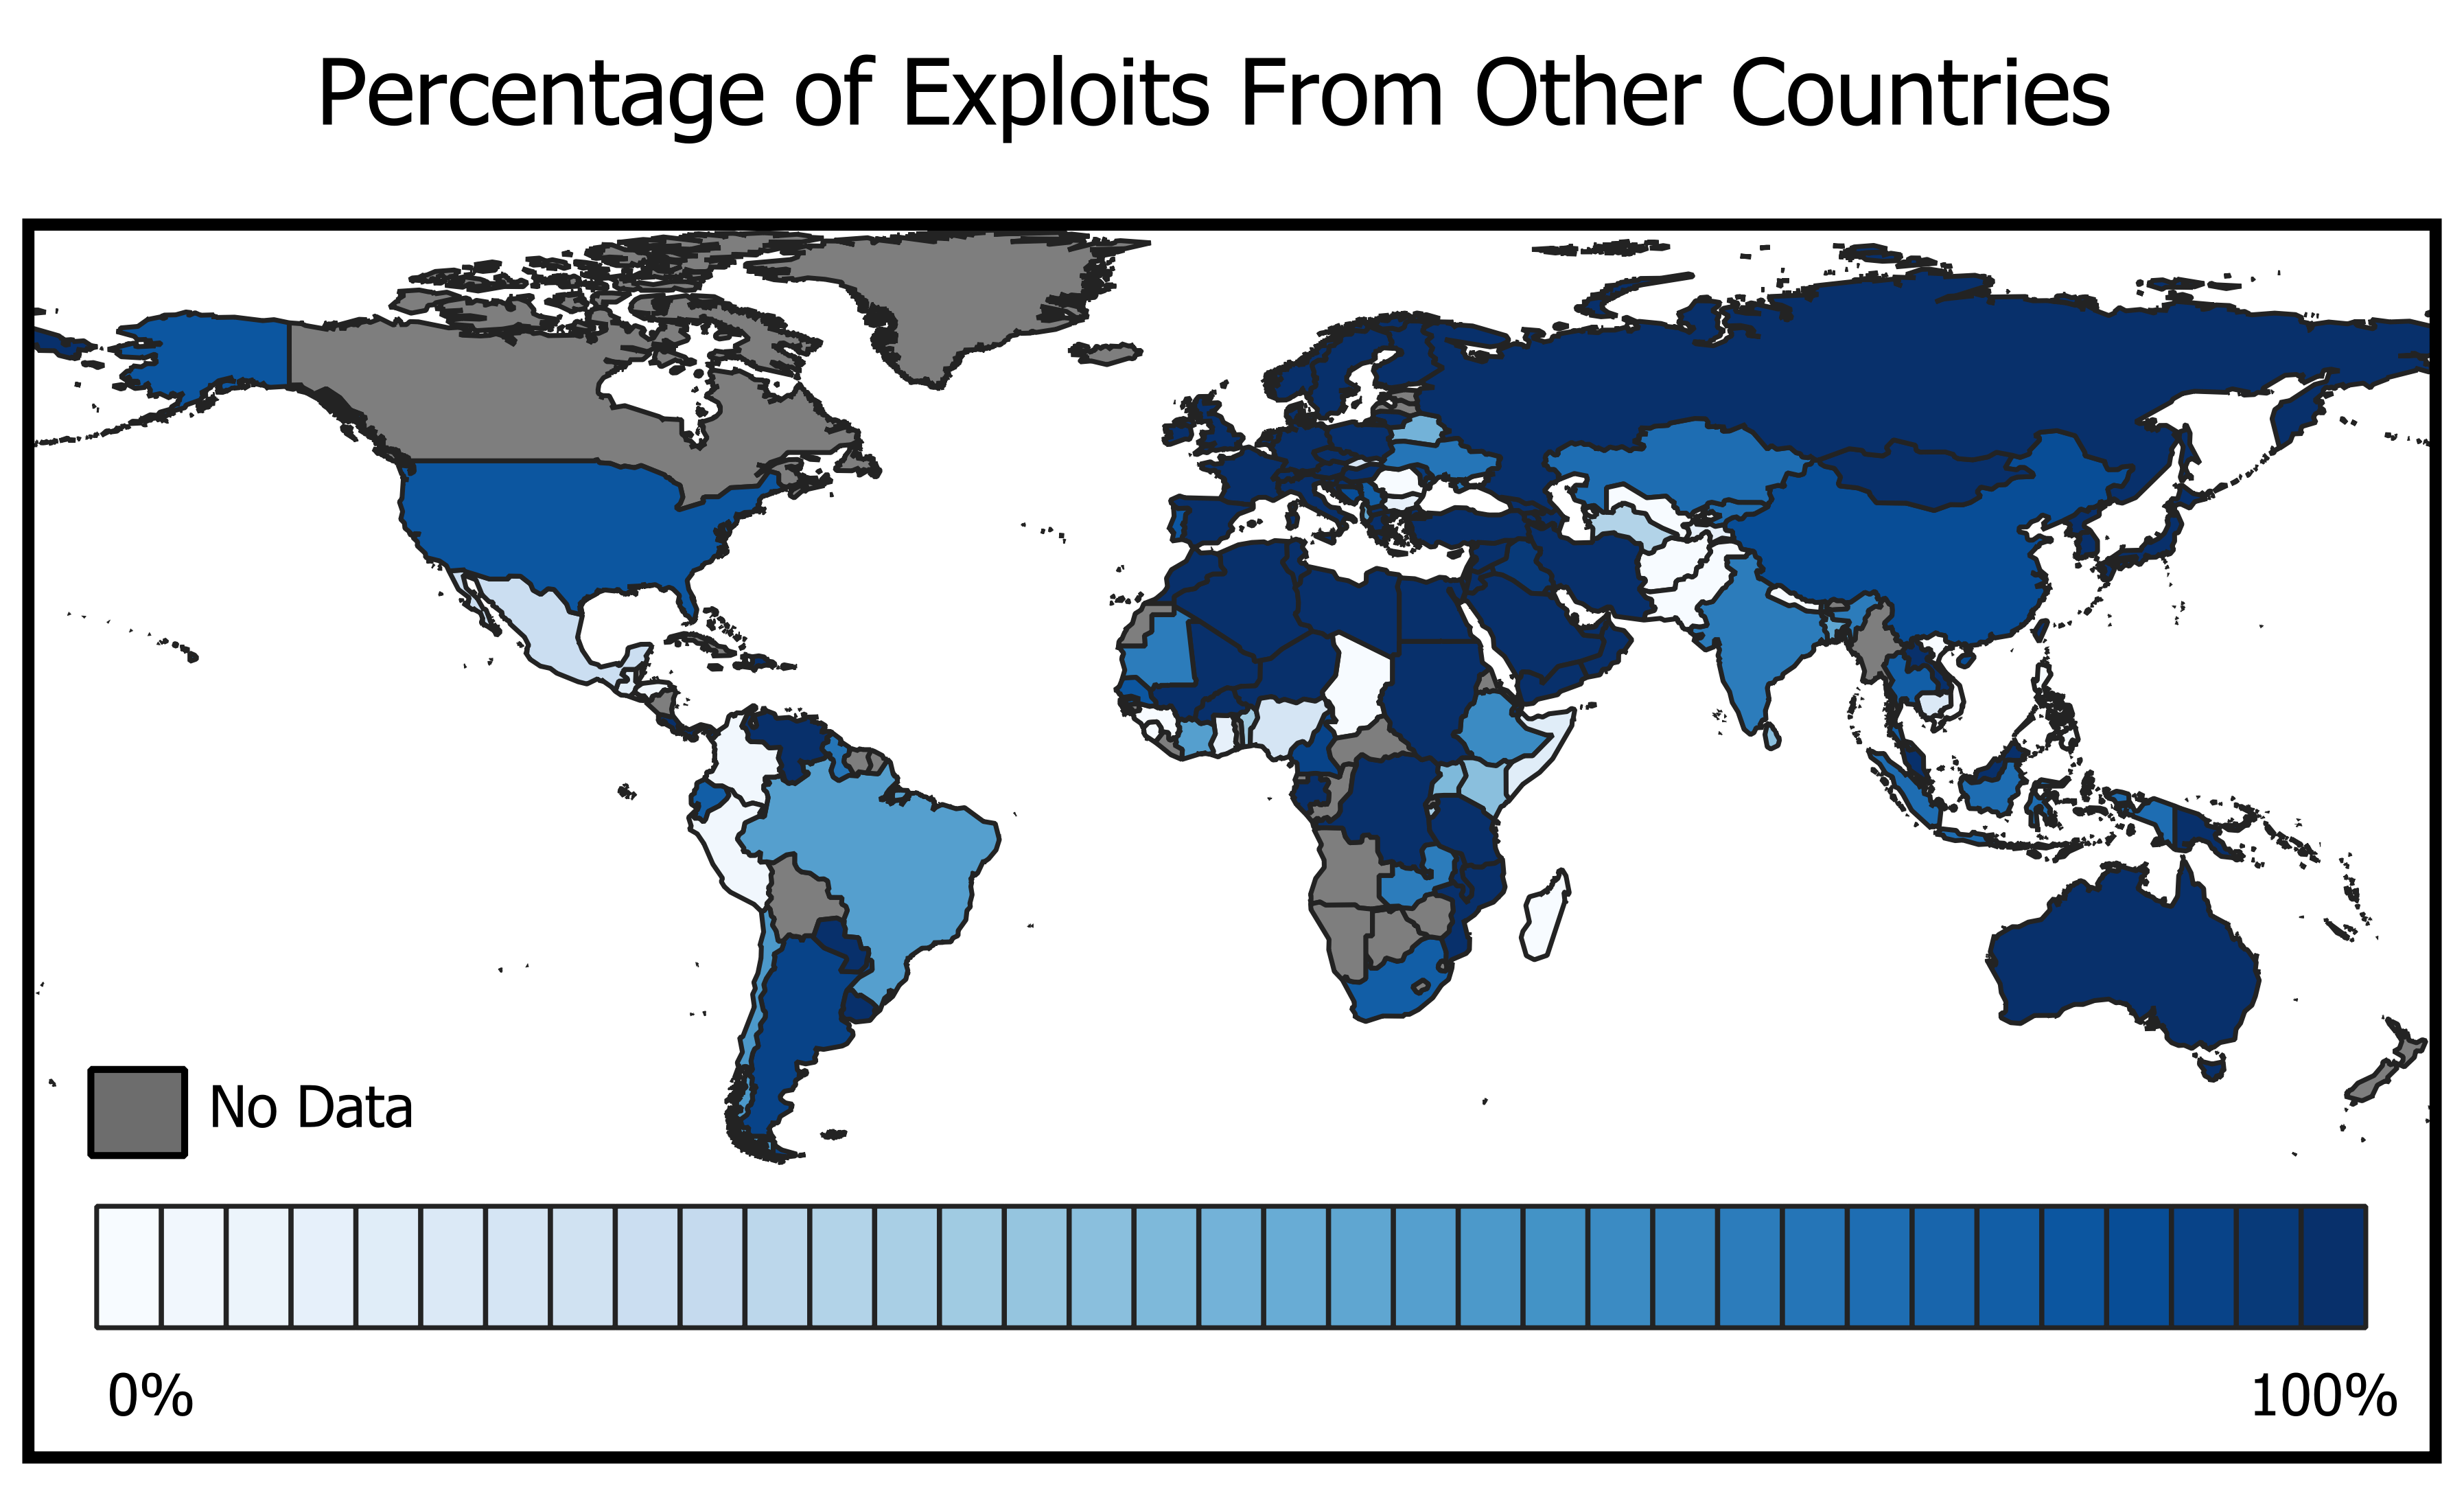
\includegraphics[width = 5.6in]{ProposalMap1}
		\scriptsize{\caption{Created with data from \cite{CTDC}}}
	\end{figure}
\end{center}
\FloatBarrier

In this map, each country is colored one of many shades of blue, where darker shades correspond to a higher percentage of international victims within the country. We can see in the map that there are a lot of dark-blue regions. Some distinctly blue regions are North-Africa and Europe. There are also some scattered regions in South-East Asia which have a high percentage of international trafficking victims. 

Of additional interest are the very light-blue or even white regions of the map. these regions have a low percentage of international trafficking victims, which means that these countries almost exclusively have victims who originate from within the country. While this visualization gives us an idea of the prevalence of international victims who are exploited in each country, it does not show us how many victims originating from a country are "exported" to other regions.

\FloatBarrier

\begin{center}
	\begin{figure}[H]
		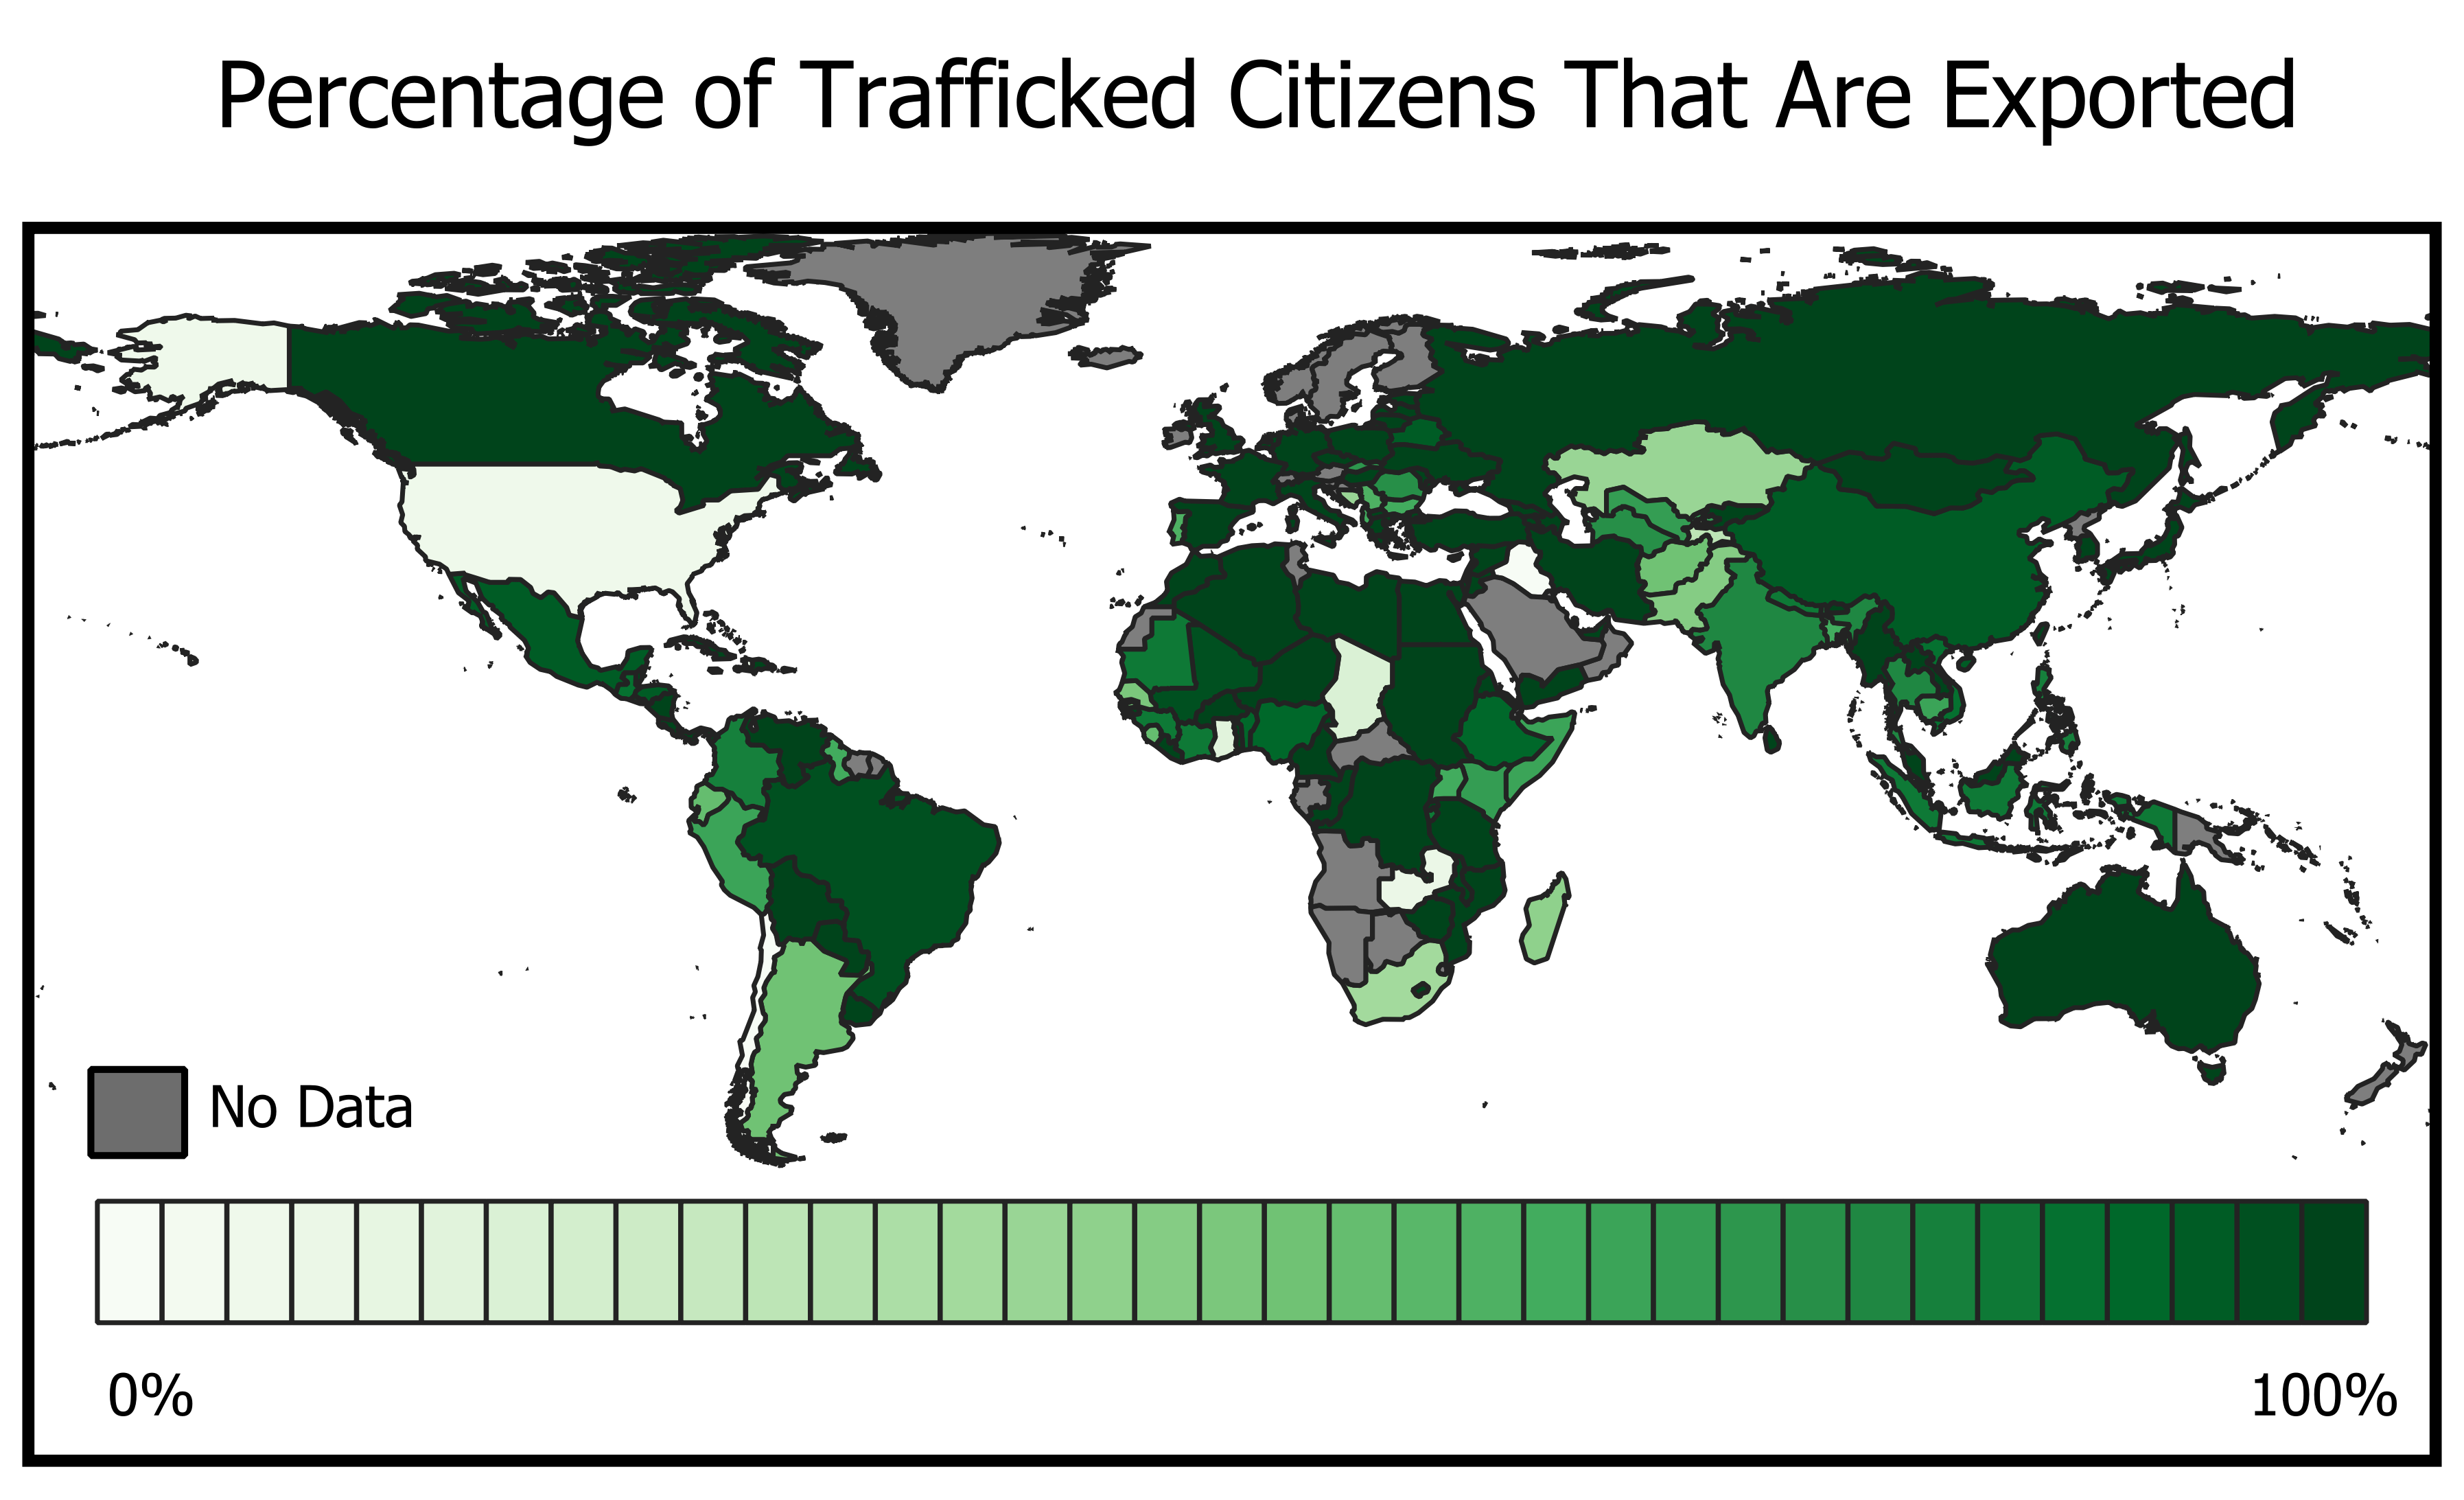
\includegraphics[width = 5.6in]{ProposalMap2}
		\scriptsize{\caption{Created with data from \cite{CTDC}}}
	\end{figure}
\end{center}
\FloatBarrier

This map is similar to the first one in that a darker color (in this case green), indicates a higher percentage of trafficked citizens who are exported from their country of origin. These two maps on their own do not paint a good picture, but when viewed together, they provide useful qualitative information.

Some preliminary conclusions one could make from these maps. For example: Mexico has a low percentage of victims from other countries, and a large percentage of Mexican citizens who are exploited, exploited in other countries. Thus we can conclude that Mexico is an "exporter" of human trafficking victims.
	
The Northern region of Africa has a high percentage of citizens that are exported, as well as a large percentage of exploits which are from other countries. This means that countries in the region displace many of their exploited citizens to other countries, but bring in victims from other countries. This suggests that individuals in North Africa are trafficked to other regions to fill a certain "role," and victims from other regions ar imported to fill a different role. In fact, we know this to be true as a result of previous studies on the region.

The smuggling of migrants and laborers from Northern Africa to Europe explains the high percenage of exploited citizens that are exported \parencite{AfricaExport}. The high percentage of victims within these countries coming from other regions is explained by the trafficking of individuals from West Africa to North Africa. Many West African migrants attempting o get to the Mediterranean Sea, are often intercepted and trafficked along their route through Algeria and Libya \parencite{AfricaImport}.

Mexico and North-Africa are just two examples of the many types of qualitative conclusions one can make from these maps; however, a major question these maps could never answer is what types of trafficking are present, what indicators exist to determine the typology of trafficking victims in a region, and most importantly, how the stage in development of a country effects these indicators and types of trafficking.



\section{Objective}

The objective of this research is to use an existing dataset, \cite{CTDC} (The CTDC Dataset), to develop models that show what types and indicators of trafficking are present in countries of different stages of development. This is a significant gap in the existing knowledge offered to law enforcement nd law makers in regards to international human trafficking. By creating these models, it will provide these entities with information more specific to the country they serve, and will allow them to make more informed decisions.

\section{Existing Research}

\subsection*{A Step Towards Modeling and Destabilizing Human Trafficking}

This article, published in 2010, is the earliest publication I could find that sought to apply machine learning to modeling human trafficking. This article talks about the large amounts of data involved in human trafficking and mentions the ways in which machine learning can be applied. 

Even in 2010, the author Shreya Amin, writes "Knowledge about the structure of a human trafficking network, from beginning of the process to the end, is extremely important and is missing." This is a statement that is still very much true today; however, now greater tools for machine learning exist but Amin's article makes it clear that this issue has been a longstanding and challenging one. 
\nocite{firstML}

\subsection*{Human Trafficking: A Perfect Storm of Contributing Factors}

This is a section of a larger book in which Susan Tiano discusses human trafficking. The reason this section is important is because it relates human trafficking to the Demographic Transition Model. This resource talks about how the rise and fall in birth and death rates has an effect on trafficking. It first talks about the growth of the "underground economy" as a whole, but focuses in on human trafficking as the chapter continues. This publication as a whole simply validates the idea that demographic transition does have an effect on human trafficking. One gap in what this publication covers is being able to quantify the effect demographic transition has. This is why creating models to quantify it would be useful.

\nocite{SlaveBook}



\section{Preliminary Reasoning and Analysis}

The Counter Trafficking Data Collaborative (CTDC) has a publicly available, anonymized dataset, which is a collection of over 400,000 entries for human trafficking victims \parencite{CTDC}. The database has plenty of useful information, such as country of citizenship, country of exploitation, and many variables expressing the type(s) of trafficking the victim experienced. This data set is what this research and models will be based on, as it is the largest publicly available database for instances of international human trafficking.

While the CTDC database is extremely large, it does not contain information on a country's development. For this, one needs a numerical way to categorize countries into "stages," as the goal is to make a generalized model for stages of development, not one that pertains to specific countries. By far the simplest way to categorize countries would be by using the Demographic Transition Model \parencite{bongaarts2009}. Using this model, a country can be categorized into one of 5 stages, with stage 1 being the lowest developed countries, and stage 5 being the most developed.

Unlike many other ways of classifying countries in terms of their development, this model uses birth, death, and migration rates to determine a country's stage \parencite{bongaarts2009}. While these rates are not directly related to a country's economic growth or decline, the model has been shown to be very successful at expressing economic changes, while not being as strongly influenced by sudden, temporary economic setbacks or "booms" \parencite{kirk1996,bar2010,galor2000}. The model has even been shown to help predict changes in the "shadow economy," in areas of illegal activity such as drug trafficking \parencite{sch1994}. It is for these reasons that I believe there exists a way to efficiently model and predict changes in the human trafficking typology of a country as it becomes more or less developed.

For our data, a complete entry is a case in which we have a value for all variables in the dataset. An incomplete entry is any entry in which there are values which are unknown, such as the age of the victim, or the type of trafficking experienced. By looking at complete entries in the CTDC Dataset, we can do a preliminary correlation comparison. We can take both the stage of the citizenship country, and exploitation country for a victim, and see if this correlates with any aspects of trafficking they experienced. The closer to perfectly correlated (-1 or 1) or connected two variables are, the more red or blue the circle will be. If a circle is red, that means the trait is seen more in low stage countries, and if it is blue, it is observed more often in high-stage countries.

\hspace*{-1.5cm}
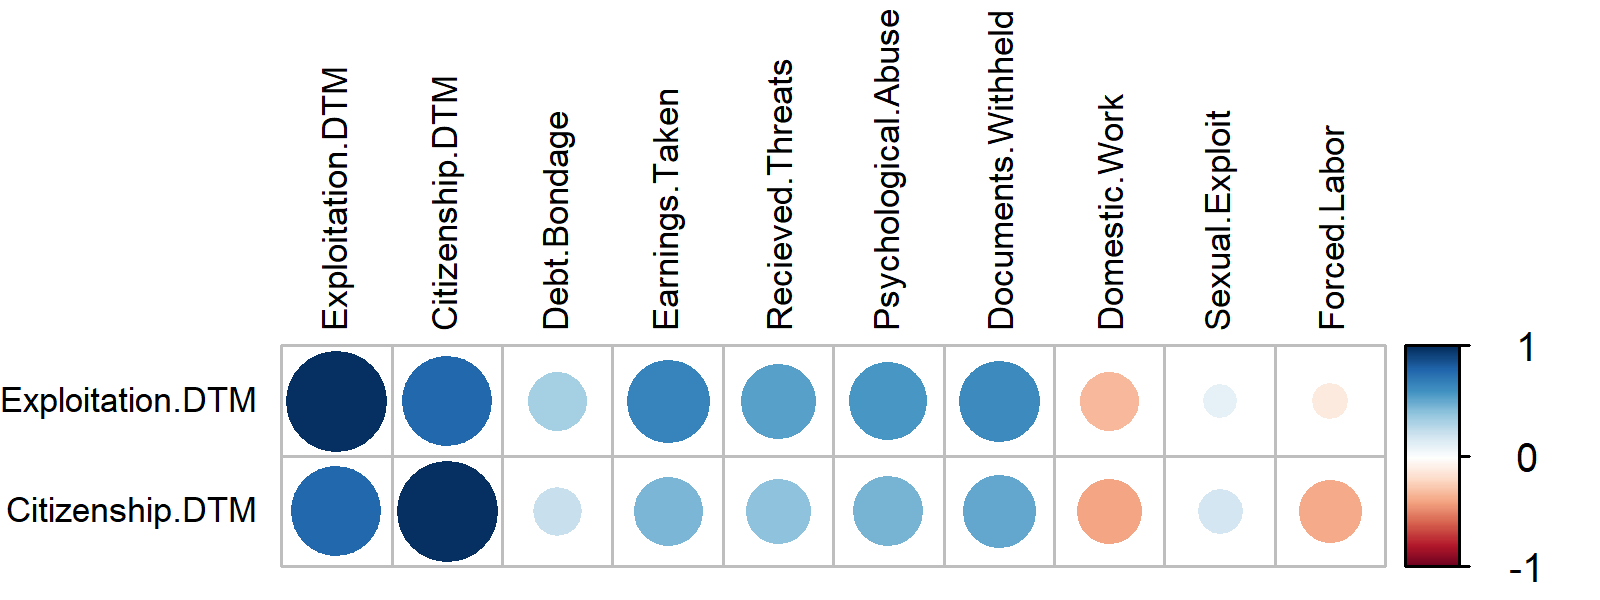
\includegraphics{Corrplot} \bigskip

Each of the variables included in the plot have at least a moderate correlation with DTM. As such, it would be beneficial to further quantify and model what types of relationships do exist within the data.


\section{Research Plan}

The eventual goal of this research is to create a multinomial regression model. This is a probabilistic model which, for any given observation, it will give the probability of the observation being in a certain group. In our case, the groups will be the stage of development of a country in which a human trafficking victim is found. By creating a model of this type, we can determine which aspects of human trafficking have the greatest correlation with the stage of development of the country. As a result, one can learn what impact a change in the level of development within a country has on the typology of human trafficking. Thus, we can quantify just how much of an effect country development has on human trafficking.

The creation of this model will initially be done using a multinomial neural-network architecture to find which coefficients for predictors provide the least number of classifications on the data. If time permits, other model architectures will be tested to see if any of those perform better on our data set.


Perhaps the biggest hurdle to be overcome is the sheer lack of complete entries in the data set. As a result, the first steps of this research will involve analyzing what data is missing, and determining how to address that. By using visualizations and quantitative measurements, we can determine which observed values (predictors) are causing the most incomplete entries in our data. We can also determine which predictors are missing in tandem, and which ones are missing independently. By doing this, we can determine which variables we should remove first, and see if it gives us enough complete observations to create a helpful model.

To test the effectiveness of our model, we will randomly split our data into two groups: a group for training the model, and a group for testing the model. After training the model, we will simply input the observations for the test set, and see how accurately the model is able to classify the observations.

\subsection{Assumptions and Limitations}


For the purposes of this research, instead of classifying an instance of human trafficking into one type or category, we will use many different categories to describe a case in the following way. We will begin by having two main categories with sub-categories. Then for each case, we will "classify" it by simply observing which of the sub categories are present. If all of the observed sub-categories fall under sex trafficking, then we can classify the case under sex trafficking. Similarly the same would happen with labor trafficking, and if a case has aspects of both, then we classify the case as "labor and sex trafficking".

\FloatBarrier
\begin{table}[htb]
	\begin{tabular}{ |p{3cm}|p{3cm}||p{3cm}|p{3cm}|  }
		\hline
		\multicolumn{4}{|c|}{Types of Human Trafficking}                                 \\ \hline
		\multicolumn{2}{|c||}{Sex Trafficking} & \multicolumn{2}{|c|}{Labor Trafficking} \\ \hline
		Prostitution    & Private Services     & Agriculture        & Aquafarming        \\
		Remote Services & Pornography          & Begging            & Construction       \\
		&                      & Domestic Work      & Hospitality        \\
		&                      & Illicit Activities & Manufacturing      \\
		&                      & Mining or Drilling & Peddling           \\
		&                      & Transportation     &                    \\ \hline
	\end{tabular}
	\caption{Types of Human Trafficking with Sub-Categories}
\end{table}
\FloatBarrier

Each example in our sub-categories, have a binary variable in the CTDC Dataset. this means that for a sub-category, the entry has a value of 0 if it is not observed, and 1 if it is. These values could also be missing, and if we determine that a variable is missing very frequently, then it may be worth removing that variable for all entries in order to have a more complete dataset. For example, if it is determined that a large percentage of entries have no entries for "Mining or Drilling," then we may remove the variable from the dataset entirely in order to create a more robust model.


\section{Final Goals}

One of the simplest explanations for why law enforcement is unequipped to adequately address human trafficking is that they "[do] not have the time,
resources or expertise to address [the] problem," \parencite{LawResponse}. The goal of this research is to produce an understanding of the types of connections that exist between certain aspects of human trafficking and how developed an area is. This would allow policy makers to create policies which allow law enforcement to be more equipped to find victims of human trafficking as their country becomes more developed, or less developed, as is the case in countries with civil unrest and have been effected by natural disasters \parencite{bar2010}.


\printbibliography


\end{document}
